\chapter{Estudo de caso - Parte II} \label{cha:estudoii}

\section{PAs analisados} \label{sec:estudoii-pas}

Neste estudo de caso foram realizadas quatro análises de forma a confirmar a viabilidade da abordagem utilizada na validação da inversa digital do PA em seu papel de pré-distorcedor digital, por meio do uso de sinais originados em diferentes PAs.

Os PAs testados foram um Si LDMOS classe AB modulado por um sinal 3GPP WCDMA e com as medições realizadas por um analisador vetorial de sinais (VSA) Agilent MXA N9020A, enquanto o PA operava com uma potência média de saída de 31,5 dBm (na sequência, este PA será designado de LDMOS{\_}AB) {\cite{franca_three-layer_2015}}, um GaN HEMT classe AB modulado por um sinal 3GPP WCDMA e com as medições realizadas por um VSA Rohde \& Schwarz FSQ (na sequência, este PA será designado de GaN{\_}AB{\_}1) {\cite{Bonfim2016}}, um GaN HEMT classe AB estimulado por duas portadoras moduladas por sinais 3GPP WCDMA e medido com um VSA Rohde \& Schwarz FSQ durante sua operação com uma potência média de saída de 26 dBm (na sequência, este PA será designado de GaN{\_}AB{\_}2) {\cite{franca_three-layer_2015}} e um GaN HEMT Doherty modulado por sinal LTE OFDMA com as medidas de entrada-saída conseguidas por meio de uma simulação do circuito operando com uma potência média de saída de 30,5 dBm (na sequência, este PA será designado de GaN{\_}Doherty) {\cite{franca_three-layer_2015}}.

\section{Ferramentas} \label{sec:estudoii-fer}

Entre as diversas ferramentas existentes para o desenvolvimento e modelagem, o Matlab se destaca dentro do ambiente acadêmico e foi escolhido para esse estudo de caso como principal ferramenta de modelagem e análise.

A função \textit{lsqnonlin} do Matlab, utilizando o algoritmo Levenberg-Marquardt \cite{Marquardt1963}, foi usada para o treinamento das redes neurais e a função \textit{fsolve}, que encontra os zeros de sistemas não-lineares de valores reais, para resolver o problema inverso.

\section{Validação do DPD por meio do PI} \label{sec:estudoii-dpd}
O método estabelecido na literatura para a validação da pré-inversa requer uma medição adicional do PA após o treinamento do DPD. Esse estudo de caso tem o objetivo de oferecer uma alternativa que emprega somente as medições do PA coletadas antes do treinamento do DPD.

O método proposto precisa da geração de um sinal de saída do pré-distorcedor que seja igual às entradas previamente medidas no PA. Uma vez que, na estratégia proposta, todas as medidas do PA são feitas antes do treinamento do DPD, o sinal de entrada do PA nunca será uma sequência pré-distorcida, sendo sempre um sinal não distorcido. Na estratégia proposta busca-se obter uma entrada do DPD que idealmente seja uma réplica da saída medida no PA que, por sua vez, é um sinal distorcido. Como mostrado na \autoref{fig:pi-validacao} o DPD e suas saídas são conhecidos, mas as entradas do DPD necessárias para gerar o sinal de saída do pré-distorcedor que seja igual às entradas do PA previamente medidas são desconhecidas. Achar estas entradas descreve um problema inverso, representado pelo bloco $DPD^{-1}$ na \autoref{fig:pi-validacao}, que precisa de uma solução numérica para cada instante de tempo.

Para finalizar a validação, o erro entre as entradas do DPD, estimadas por meio da solução do problema inverso, e as saídas previamente medidas do PA é computado. Isso é equivalente a medir o erro entre a entrada da cascata e o sinal de saída, como mostrado na \autoref{fig:pi-validacao}. Visto que a saída da cascata deve apresentar uma relação linear com a sua entrada, o erro computado é uma medida da capacidade de linearização do sinal pelo DPD.

\imagem{PI proposta para validar o DPD}{
\resizebox{0.8\textwidth}{!}{
\centering
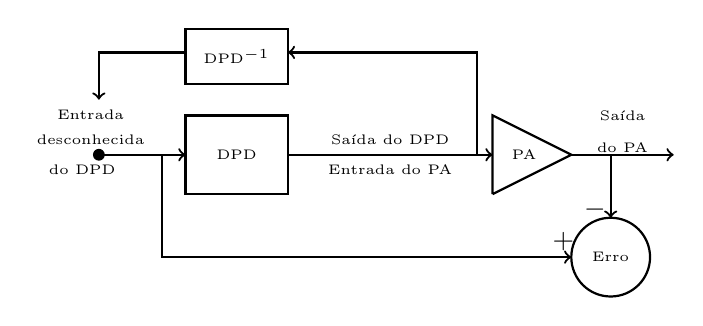
\begin{tikzpicture}[->,thick]
  \draw  (-2.5,1.5) rectangle node {\tiny DPD} (-1.2,0.5);
  \draw  (2.9,-0.3) ellipse (0.5 and 0.5) node {\tiny Erro};
  \draw (-3.6,1)  node[above, xshift=-3,yshift=9] {\tiny Entrada}  node[above,xshift=-3] {\tiny desconhecida} node[below,xshift=-6] {\tiny do DPD}-- (-2.5,1);
  \draw (-2.8,1) -- (-2.8,-0.3) -- (2.4,-0.3);
  \draw (-1.2,1) -- node[above] {\tiny Saída do DPD} node[below] {\tiny Entrada do PA} (1.4,1);
  \draw (2.4,1) -- node[above, align=center,yshift=0.3cm] {\tiny Saída} node[above,yshift=-0.1cm] {\tiny do PA} (3.7,1);
  \draw (2.9,1) -- (2.9,0.2);
  \node[circle, fill,minimum size=1.5mm,inner sep=0pt,outer sep=0pt] at (-3.6,1) {};
  \draw[-] (1.4,0.5) -- (1.4,1.5) -- (2.4,1) -- (1.4,0.5);
  \node at (1.8,1) {\tiny PA};
  \node at (2.3,-0.1) {$+$};
  \node at (2.7,0.3) {$-$};
\draw (1.2,1) -- (1.2,2.3) -- (-1.2,2.3);
\draw  (-1.2,2.6) rectangle node {\tiny DPD$^{-1}$} (-2.5,1.9);
\draw (-2.5,2.3) -- (-3.6,2.3) -- (-3.6,1.7);
\end{tikzpicture}
}
\label{fig:pi-validacao}
}{O autor}{fig:pi-validacao}{}{Diagrama de blocos com as conexões presentes entre os blocos do DPD, da inversa do DPD e do PA para o processo de validação do DPD através do uso do problema inverso.}

\section{Estratégia Proposta} \label{sec:estudoii-2}
Na técnica tradicional de validação um sinal de entrada conhecido é processado pelo modelo de DPD para se extrair um sinal de saída, o sinal de saída é então passado pelo PA de forma a produzir uma replica linear do sinal de entrada. Em tal problema direto, a incógnita é a amostra instantânea de saída do DPD $out_{DPD}(n)$, que é uma função explícita das amostras presentes e passadas da entrada do DPD, de acordo com:
\begin{equation}
\small out_{DPD}(n)=f[in_{DPD}(n),\ldots, in_{DPD}(n-M)].
\label{implicit_01}
\end{equation}

Na técnica proposta de validação o sinal de entrada do DPD é desconhecido e precisa ser encontrado, enquanto todos os outros sinais na cascata são conhecidos. O DPD é validado analisando o erro entre o sinal de entrada encontrado pela resolução do problema inverso e o sinal conhecido da saída da cascata. Em tal problema inverso, a incógnita é a amostra de entrada instantânea do DPD $in_{DPD}(n)$, que só pode ser escrita como uma função das amostras de saída instantâneas do DPD e das amostras de entradas passadas na sua forma implícita, de acordo com:
\begin{equation}
\small g[in_{DPD}(n),\ldots, in_{DPD}(n-M), out_{DPD}(n)]=0.
\label{implicit_02}
\end{equation}

Para resolver o problema inverso em sua forma implícita, os zeros da equação algébrica não-linear da \autoref{implicit_02} precisam ser encontrados. Pelo motivo da \autoref{implicit_02} manipular sinais de amostras passadas, para cada instante de tempo uma equação não-linear distinta é obtida. Consequentemente, a \autoref{implicit_02} precisa ser resolvida para cada instante de tempo em uma ordem sequencial. A solução da \autoref{implicit_02} é um número de valor complexo que pode ser separado em parte real e imaginária. Além disso, a \autoref{implicit_02}, de valores complexos, é equivalente a impor que as partes reais e imaginárias do operador \textit{g} são simultaneamente zero.

\section{Resultados} \label{sec:estudoii-3}

Na \autoref{tab:sinais_med1} são apresentadas a frequência central ($f_{c}$) de operação do sinal, a largura de banda (BW) e a diferença entre a frequência central da faixa central e as frequências centrais das faixas adjacentes ($\Delta f_{cen}$).
\tabela{Informações dos sinais dos PAs}{
\begin{tabular}{c|c|c|c}
\hline
    \textbf{PA} & \textbf{$f_{c}$ (GHz)} & \textbf{BW (MHz)} & \textbf{$\Delta f_{cen}$ (MHz)}\\\hline 
    LDMOS{\_}AB  & 2 & 3,84 & 5\\\hline
    GaN{\_}AB{\_}1  & 0,9 & 3,84 & 5\\\hline 
    GaN{\_}AB{\_}2 & 0,9 & 8,84 & 10\\\hline 
    GaN{\_}Doherty & 2,14 & 7,68 & 10\\\hline
\end{tabular}
\label{tab:sinais_med1}
}{O autor}{tab:sinais_med1}{}{Informações da frequência central, largura de banda e tamanho da faixa adjacente a frequência central para os quatro PAs analisados.}

A \autoref{tab:sinais_med2} relativa a medição e obtenção do sinal, aponta a frequência de amostragem ($f_{s}$) utilizada, o número de amostras para o conjunto de dados de treinamento e o número de amostras para o conjunto de dados da validação.
\tabela{Informações da amostragem dos PAs}{
\begin{tabular}{c|c|c|c}
    \hline
    \textbf{PA} & \textbf{$f_{s}$ (MHz)} & \textbf{Treinamento} & \textbf{Validação} \\ \hline
    LDMOS{\_}AB  & 30,72 & 26180 & 8501 \\\hline
    GaN{\_}AB{\_}1  & 30,72 & 3221 & 2001 \\\hline 
    GaN{\_}AB{\_}2 & 61,44 & 24180 & 9600 \\\hline 
    GaN{\_}Doherty & 61,44 & 20290 & 4500 \\\hline
\end{tabular}
\label{tab:sinais_med2}
}{O autor}{tab:sinais_med2}{}{Informações da frequência de amostragem e total de amostras de treinamento e de validação para os quatro PAs analisados.}

A arquitetura baseada em TLP da \autoref{fig:model-topo} foi selecionada para todos os casos como modelo de DPD. Os dois parâmetros de ajuste da arquitetura foram a profundidade de memória \textit{M} e o número de neurônios \textit{N} presentes na camada oculta do TLP. A \autoref{tab:parametros_nn} apresenta os pares de parâmetros utilizados para cada um dos casos analisados.
\tabela{Parâmetros dos modelos de PoD/DPD}{
\begin{tabular}{c|c|c}
    \hline
    \textbf{PA} & \textbf{\textit{M}} & \textbf{\textit{N}} \\ \hline 
    LDMOS{\_}AB & 2 & 8 \\ \hline 
    GaN{\_}AB{\_}1 & 8 & 3 \\ \hline 
    GaN{\_}AB{\_}2 & 3 & 7 \\ \hline 
    GaN{\_}Doherty & 1 & 8 \\ \hline
\end{tabular}
\label{tab:parametros_nn}
}{O autor}{tab:parametros_nn}{}{Parâmetros utilizados nas redes neurais que modelam os DPDs, sendo \textit{M} a profundidade de memória e \textit{N} o número de neurônios na camada oculta.}

As rotinas de treinamento e validação não apresentam entre si diferenças em suas estruturas de processamento e nem em relação aos parâmetros das funções de otimização presentes no Matlab. Alteram-se somente as dimensões das matrizes usadas para representar as entradas e os coeficientes das redes neurais utilizadas, ajustes que são realizados com a simples alteração dos valores \textit{M} e \textit{N} durante o processo de chamada da função.

O NMSE foi empregado na validação dos modelos de PoD e DPD. No que concerne à validação do PoD, \textit{O} é a medição da entrada do PA e \textit{Ô} é a saída estimada do PoD. No que concerne à validação do DPD, \textit{O} é a medição da saída do PA e \textit{Ô} é a estimativa da entrada do DPD. A \autoref{tab:NMSE_PoD} mostra o resultado do NMSE para a validação dos modelos PoD.
\tabela{NMSE para os modelos na função de PoD}{
\begin{tabular}{c|c|c|c|c}
    \hline
    \textbf{NMSE {(dB)}} & \textbf{LDMOS{\_}AB} & \textbf{GaN{\_}AB{\_}1} & \textbf{GaN{\_}AB{\_}2} & \textbf{GaN{\_}Doherty} \\ \hline 
    Treinamento &-40,8 & -37,1 &-38,0 &-34,5 \\ \hline 
    Validação &-40,7 & -37,5 &-37,3 &-34,4\\ \hline
\end{tabular}
\label{tab:NMSE_PoD}
}{O autor}{tab:NMSE_PoD}{}{NMSE para os conjuntos de treinamento e validação na modelagem comportamental do PoD.}

A função \textit{fsolve} do Matlab é usada para resolver o problema inverso. Os valores padrões são usados, exceto pelas tolerâncias de passo e função, que recebem os valores de {$10^{-12}$}. O valor inicial para o instante \textit{n} é o valor estimado para o instante \textit{n}-1.

Além de utilizar-se o NMSE como métrica para avaliação da fidelidade do sinal estimado para a entrada do DPD em relação ao sinal de saída do PA, calculou-se a razão de potência de canal adjacente (ACPR) para o sinal estimado, conforme a seguinte definição de ACPR:
\begin{equation}
ACPR = 10\log_{10}\frac
{\int_{adj}\abs{f(\omega)}^{2}}
{\int_{cen}\abs{f(\omega)}^{2}}.
\label{acprdisc_int}
\end{equation}

Com a discretização do sinal necessária para seu processamento digital, tem-se a operação de integração transformada em um somatório:
\begin{equation}
ACPR = 10\log_{10}\frac
{\sum_{adj}\abs{f(\omega)}^{2}}
{\sum_{cen}\abs{f(\omega)}^{2}},
\label{acprdisc}
\end{equation}
onde $f(\omega)$ é o sinal no domínio da frequência e \textit{adj} e \textit{cen} referem-se, respectivamente, às faixas de frequências adjacentes, superior e inferior, e à faixa de frequências centrais do sinal. Têm-se, portanto, dois diferentes valores de ACPR para o sinal analisado, o primeiro referenciando-se à faixa adjacente superior e o segundo à inferior.

Os resultados em NMSE e ACPR obtidos para os casos analisados são apresentados na \autoref{tab:NMSE_ACPR_DPD}.
\tabela{Informações do sinal estimado pelo PI}{
\begin{tabular}{c|c|c|c}
    \hline
    \textbf{PA} & \textbf{NMSE {(dB)}} & \textbf{$ACPR_{sup}$ {(dB)}} & \textbf{$ACPR_{inf}$ {(dB)}}\\ \hline 
    LDMOS{\_}AB & -41,0 & -35,1 & -37,5\\ \hline 
    GaN{\_}AB{\_}1 & -39,3 & -29,2 & -27,5\\ \hline 
    GaN{\_}AB{\_}2 & -39,7 & -29,7 & -26,6\\ \hline 
    GaN{\_}Doherty & -36,9 & -24,6 & -24,6\\ \hline
\end{tabular}
\label{tab:NMSE_ACPR_DPD}
}{O autor}{tab:NMSE_ACPR_DPD}{}{Valores de NMSE para a validaçao da inversa do PA na função de DPD e ACPR obtidos para os casos analisados.}

Para oferecer um referencial aos valores de ACPR obtidos para os sinais estimados para a entrada das cascatas, na \autoref{tab:ACPR_SAIDA} são mostrados os valores de ACPR calculados para os sinais conhecidos das saídas das cascatas.

A \autoref{fig:bf-dpd} mostra, para cada um dos casos analisados, a amplitude da saída do PA e a diferença de fase (entre os sinais de entrada e de saída da cascata) como funções da amplitude de entrada do DPD.

A \autoref{fig:bf-psd} mostra as densidades espectrais de potência (PSDs) medidas nas saídas dos PAs (em cor preta) e estimadas nas entradas dos DPDs como soluções dos problemas inversos (as faixas centrais de frequências estão indicadas na cor azul e as faixas adjacentes na cor vermelha).


\begin{figure}[H]
\centering
\subfloat[LDMOS{\_}AB]{
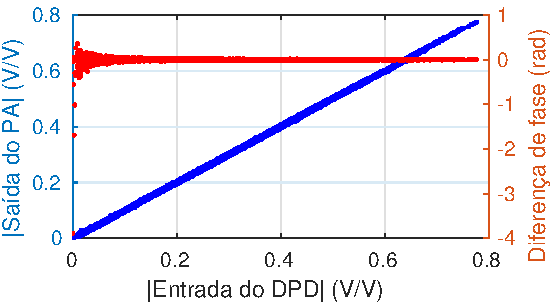
\includegraphics[scale=0.9]{fig2/fig_dpd_ldmos.pdf}
\label{fig:bf-dpd_ldmos}
}\\
\subfloat[GaN{\_}AB{\_}1]{
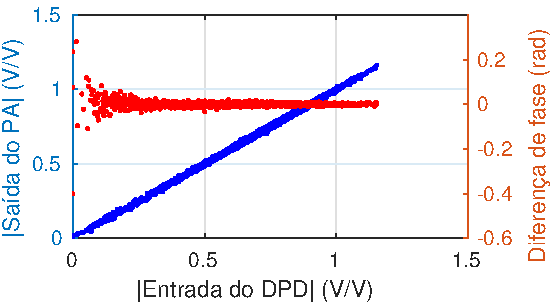
\includegraphics[scale=0.9]{fig2/fig_dpd_sbrt2.pdf}
\label{fig:bf-dpd_sbrt2}
}\\
\subfloat[GaN{\_}AB{\_}2]{
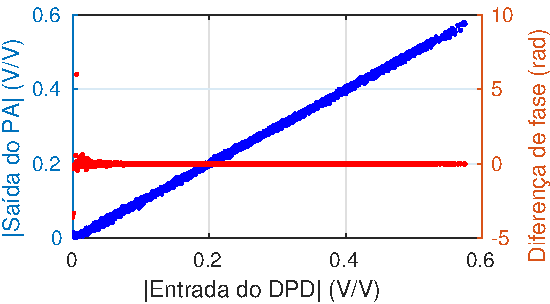
\includegraphics[scale=0.9]{fig2/fig_dpd_tc.pdf}
\label{fig:bf-dpd_tc}
}\\
\subfloat[GaN{\_}Doherty]{
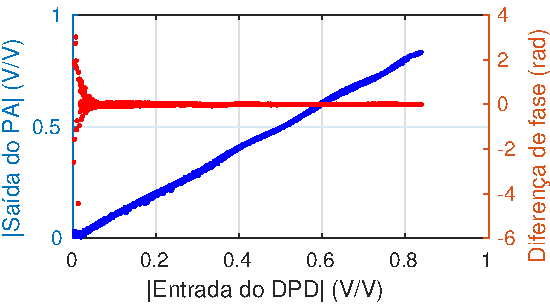
\includegraphics[scale=0.9]{fig2/fig_dpd_doherty.pdf}
\label{fig:bf-dpd_doherty}
}
\caption{Amplitude de saída do PA e diferença de fase na cascata em função da amplitude de entrada do DPD para os diferentes PAs.}
\label{fig:bf-dpd}
\end{figure}


\begin{figure}[H]
\centering
\subfloat[LDMOS{\_}AB]{
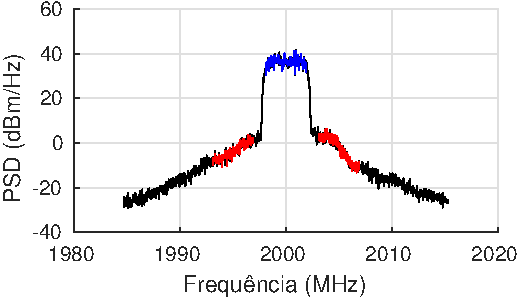
\includegraphics[scale=0.9]{fig2/Frequencia_extraction_ldmos.pdf}
\label{fig:bf-psd_ldmos}
}\\
\subfloat[GaN{\_}AB{\_}1]{
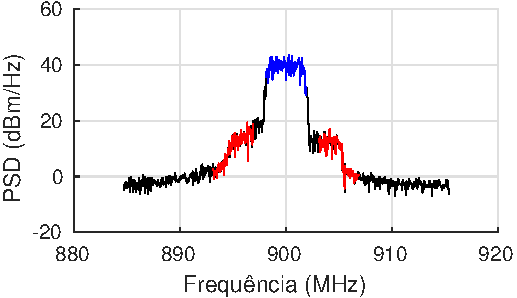
\includegraphics[scale=0.9]{fig2/Frequencia_extraction_sbrt2.pdf}
\label{fig:bf-psd_sbrt2}
}\\
\subfloat[GaN{\_}AB{\_}2]{
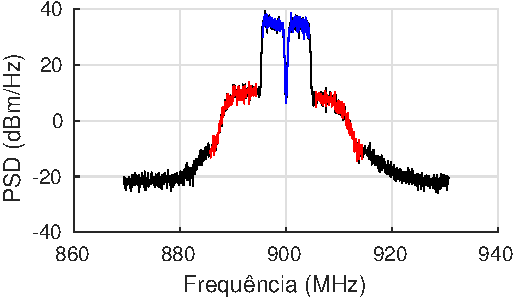
\includegraphics[scale=0.9]{fig2/Frequencia_extraction_tc.pdf}
\label{fig:bf-psd_tc}
}\\
\subfloat[GaN{\_}Doherty]{
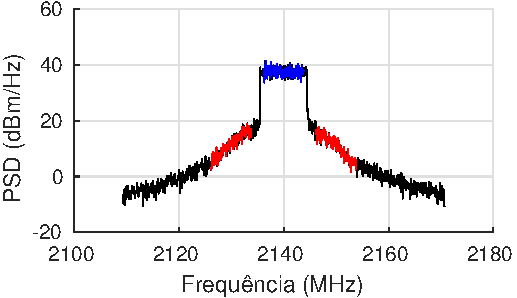
\includegraphics[scale=0.9]{fig2/Frequencia_extraction_doherty.pdf}
\label{fig:bf-psd_doherty}
}\\
\caption{PSD para as entradas estimadas dos DPDs e as saídas medidas dos PAs, considerando-se os conjuntos de dados de treinamento.}
\label{fig:bf-psd}
\end{figure}



\tabela{ACPR da saída da cascata DPD-PA}{
\begin{tabular}{c|c|c}
\hline
    \textbf{PA} & \textbf{$ACPR_{sup}$ (dB)} & \textbf{$ACPR_{inf}$ (dB)}\\ \hline 
    LDMOS{\_}AB & -35,0 & -37,5\\ \hline 
    GaN{\_}AB{\_}1 & -29,2 & -27,3\\ \hline 
    GaN{\_}AB{\_}2 & -29,6 & -26,4\\ \hline 
    GaN{\_}Doherty & -24,5 & -24,6\\ \hline
\end{tabular}
\label{tab:ACPR_SAIDA}
}{O autor}{tab:ACPR_SAIDA}{}{Valores de ACPR calculados para os sinais conhecidos da saída das cascatas DPD-PA.}

Uma avaliação mais criteriosa entre a abordagem tradicional e a proposta, especificamente para o conjunto de casos analisados nesta seção, se vê impossibilitada pela falta de medições experimentais realizadas nos PAs após a identificação dos modelos de DPD apresentados. Nestas medições não disponíveis, sequências pré-distorcidas, geradas por meio da passagem de sinais pelos DPDs correspondentes, seriam aplicadas como entradas a cada PA de maneira a se conseguir um conjunto de dados de entrada e de saída para cada uma das cascatas analisadas.

A disponibilidade destes dados é uma condição necessária para a realização de uma comparação entre os resultados da validação dos modelos pelo método tradicional e pelo método apresentado nesse trabalho. No entanto, é possível afirmar o sucesso do método de validação proposto devido aos comportamentos lineares, apresentados na \autoref{fig:bf-dpd}, entre a entrada e a saída das cascatas em função da amplitude de entrada.

Para todas as cascatas reportadas na \autoref{fig:bf-dpd}, verificam-se ganhos unitários entre a amplitude de saída e a amplitude de entrada, ilustrados pelas retas de inclinações unitárias em azul. Pela \autoref{fig:bf-dpd} observa-se também que os sinais de entrada e saída de todas as cascatas possuem praticamente a mesma fase, o que é evidenciado pelas retas horizontais em vermelho. De fato, qualquer PA construído fisicamente vai induzir algum atraso e, uma vez que o DPD é um sistema causal, a saída do PA é sempre uma versão atrasada do sinal de entrada do DPD.

Dessa forma, as medições do sinal de entrada e saída foram sempre realizadas em diferentes instantes de tempo. Como consequência, não é possível estimar o atraso absoluto do PA. Diante disso, os dados medidos foram pré-processados através do uso de algoritmos de correlação de tal forma a eliminar o atraso entre as sequências de entrada e saída do PA. Somente após a realização deste procedimento é que os sinais foram aplicados para a identificação e validação dos DPDs, o que justifica a ausência de atraso entre os sinais de saída e entrada das cascatas reportadas na \autoref{fig:bf-dpd}.

Corroborando o resultado gráfico, os valores de NMSE apresentados na \autoref{tab:NMSE_PoD} são próximos dos valores mostrados na \autoref{tab:NMSE_ACPR_DPD}, o que é um indicativo adicional de que os modelos inversos desenvolvidos comportam-se de maneira similar antes ou após os PAs nas cascatas.

Além disso, a exatidão do método de validação proposto pode ser verificada pela \autoref{fig:bf-psd} onde observa-se que, em todos os quatro estudos de caso investigados, as distorções presentes nos canais adjacentes das entradas estimadas dos DPDs através das soluções dos problemas inversos são visivelmente muito próximas das distorções medidas nos canais adjacentes das saídas dos PAs. Especificamente, analisando os resultados de ACPR reportados nas \autoref{tab:NMSE_ACPR_DPD} e \autoref{tab:ACPR_SAIDA}, observa-se que a diferença entre os valores de ACPR nas entradas e saídas das cascatas são sempre iguais ou inferiores a 0,2 dB.

\section{Comparação com a Abordagem Tradicional} \label{sec:compara}

Existindo a necessidade da comparação entre a metodologia tradicional e aquela proposta neste trabalho, uma nova análise foi realizada. Esta análise utiliza os dados medidos experimentalmente em um PA linearizado por um DPD já validado pela abordagem tradicional e compara estes resultados com os obtidos por meio da abordagem proposta.

O PA selecionado para o estudo de caso adicional foi um PA GaN classe AB, estimulado por uma portadora em 900 MHz modulada por um sinal WCDMA 3GPP com uma largura de banda de 3,84 MHz e cuja potência média de saída foi de 26 dBm para a extração dos dados. Foram utilizadas 28.800 amostras para o treinamento do modelo e 8.700 amostras para a validação, sendo a frequência de amostragem de 61,44 MHz e as medições realizadas por meio de um VSA Rohde \& Schwarz FSQ \cite{lima2009rfpa}.

O modelo de DPD correspondente ao PA foi projetado utilizando-se o modelo polinomial descrito pela seguinte equação:
\begin{equation}
\tilde{y}(n) = \sum\limits_{p=1}^{P_0} \sum\limits_{m=0}^{M}\tilde{b}_{p,m}|\tilde{x}(n-m)|^{p-1}\tilde{x}(n-m),
\label{dpdcomp}
\end{equation}
na qual $\tilde{y}(n)$ representa a enésima saída do DPD, $\tilde{x}(n)$ a enésima entrada do DPD, $P_{0}$ a ordem do polinômio resultante, \textit{M} a profundidade de memória requerida pelo polinômio e $\tilde{b}_{p,m}$ é o conjunto de coeficientes que serão ajustados pelo método dos mínimos quadrados de forma a modelar a pré-inversa do PA, sendo definida a ordem do polinômio resultante $P_{0}$ como 7 e a profundidade de memória \textit{M} como 3.

Dois conjuntos de dados diferentes foram utilizados para esta comparação. O primeiro deles é formado pelos valores de entrada e saída da cascata e foi utilizado para a obtenção dos valores de NMSE e ACPR referentes a validação tradicional, assim como para a obtenção da \autoref{fig:abr_trad}. Em outras palavras, para a obtenção deste primeiro conjunto de dados, uma nova medição do PA foi realizada após o treinamento do DPD, no qual um sinal conhecido foi primeiramente aplicado na entrada do DPD e a sequência pré-distorcida gerada pelo DPD foi então aplicada na entrada do PA. O segundo conjunto de dados é formado pelos valores de entrada e saída do PA medidos antes da identificação do DPD e foi utilizado para a obtenção dos valores de NMSE e ACPR referentes ao método proposto de validação e também para a obtenção da \autoref{fig:abr_prp}.

O cálculo do ACPR foi realizado para os sinais de entrada e saída das cascatas. Foi utilizada uma diferença entre a frequência central da faixa central e as frequências centrais das faixas adjacentes de 5 MHz.

Na \autoref{tab:nmse_comp} são comparados os valores de NMSE e ACPR. Verifica-se através da análise do NMSE que o resultado da metodologia proposta apresenta uma estimativa mais conservadora em relação à realidade, uma consequência do erro adicional ao sistema pela resolução do problema inverso. Pela \autoref{tab:nmse_comp}, verifica-se que os valores de ACPR obtidos na entrada e saída da cascata que valida o DPD usando a estratégia proposta são mais próximos entre si do que os respectivos valores para a cascata que valida o DPD usando a estratégia tradicional. Em específico, na cascata que valida o DPD por meio da estratégia proposta, as diferenças de ACPR de entrada e saída são de no máximo 4,0 dB, enquanto que na cascata que valida o DPD por meio da estratégia tradicional, as diferenças de ACPR de entrada e saída são de até 21,5 dB.

Cumpre ressaltar que, na estratégia tradicional busca-se estimar valores extremamente baixos de ACPR, o que de fato configura-se em uma tarefa muito difícil de ser cumprida. Dessa forma, pode-se concluir que, em ambas as estratégias, o objetivo de obter um sinal de saída da cascata que seja uma réplica do sinal de entrada da cascata é cumprido de maneira bastante satisfatória.
\tabela{Comparação de NMSE e ACPR entre as abordagens}{
\begin{tabular}{c|c|c}
    \hline 
    \textbf{Abordagem} & \textbf{Tradicional} & \textbf{Proposta}\\ \hline 
    NMSE (dB) & -44,6 & -38,9 \\\hline
    $ACPR_{sup}$ de Entrada (dB) & -77,2 & -36,0 \\ \hline 
    $ACPR_{inf}$ de Entrada (dB) & -77,8 & -33,6 \\ \hline 
    $ACPR_{sup}$ de Saída (dB) & -57,9 & -39,1 \\ \hline 
    $ACPR_{inf}$ de Saída (dB) & -56,3 & -37,6 \\ \hline 
\end{tabular}
\label{tab:nmse_comp}
}{O autor}{tab:nmse_comp}{}{Valores de NMSE e ACPR para a comparação entre as duas abordagens.}

Na FIGURA\autoref{fig:abr_txp} são observados tanto o comportamento linear necessário como a pequena diferença de fase, condições necessárias para o bom funcionamento do DPD.

\imagemHH{Comparação entre métodos}{
\subfloat[Tradicional]{
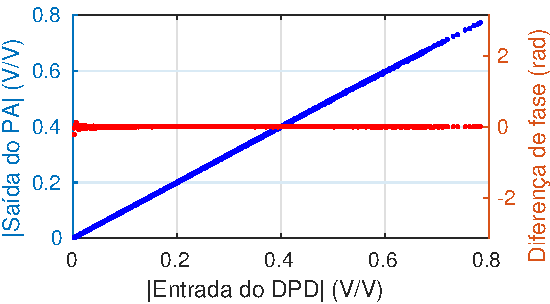
\includegraphics[scale=0.9]{fig2/fig_dpd_trad.pdf}
\label{fig:abr_trad}
}
\hspace{0.5cm}
\subfloat[Proposto]{
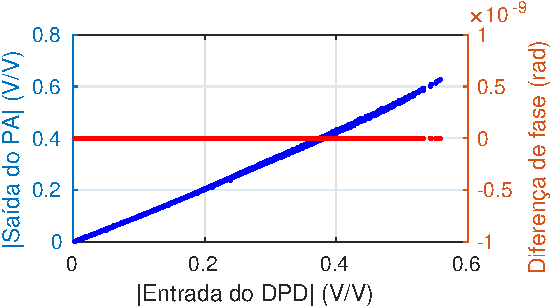
\includegraphics[scale=0.9]{fig2/fig_dpd_new.pdf}
\label{fig:abr_prp}
}
\label{fig:abr_txp}
}{O autor}{}{}{Amplitude de saída do PA e diferença de fase na cascata em função da amplitude de entrada do DPD para: a) Método tradicional de validação; b) Método proposto de validação.}
